\documentclass[10pt,letterpaper]{article}

%% ──────────────────────────────────────────────────────
%%  PNAS-style single-column template
%% ──────────────────────────────────────────────────────
\usepackage[top=2.5cm, bottom=2.5cm, left=2.8cm, right=2.8cm]{geometry}
\usepackage{amsmath,amssymb}
\usepackage{graphicx}
\usepackage{booktabs}
\usepackage{array}
\usepackage{longtable}
\usepackage[hidelinks,colorlinks=true,linkcolor=blue,citecolor=blue,urlcolor=blue]{hyperref}
\usepackage{natbib}
\usepackage{xcolor}
\usepackage{microtype}
\usepackage{setspace}
\usepackage{parskip}
\usepackage{titlesec}
\usepackage{caption}
\usepackage{subcaption}
\usepackage{footnote}
\usepackage{url}
\usepackage{float}
\usepackage{tikz}
\usetikzlibrary{shapes.geometric, arrows.meta, positioning}
\usepackage{CJKutf8}
\usepackage{fontenc}
\usepackage{inputenc}

%% ── Typography ───────────────────────────────────────
\setstretch{1.10}
\setlength{\parskip}{4pt}

\titleformat{\section}{\normalfont\bfseries\large}{}{0em}{}[\titlerule]
\titleformat{\subsection}{\normalfont\bfseries\normalsize}{}{0em}{}
\titleformat{\subsubsection}{\normalfont\itshape\normalsize}{}{0em}{}

\captionsetup{font=small, labelfont=bf, skip=4pt}

%% ── Title block ─────────────────────────────────────
\title{\textbf{What Do Retired Athletes Fight For?\\
Topic Modeling of Court Complaints Against China's\\
Whole-Nation Athlete Development System}}

\author{
  Wangyixun (Frances) Jiang\\
  \small QSS 20 · Dartmouth College · Spring 2026
}
\date{}

%% ─────────────────────────────────────────────────────
\begin{document}
\maketitle
\thispagestyle{empty}

\begin{abstract}
\noindent
China's \textit{jǔguó tǐzhì} (``Whole-Nation System'') produces Olympic champions through state-funded, full-immersion sports schools, but its retirement welfare mechanisms remain understudied. Using Latent Dirichlet Allocation (LDA) topic modeling on 79 court cases from China Judgements Online---the Supreme People's Court's official public case database---I identify the principal areas of complaint raised by retired Chinese athletes against the system. Eight topics emerge from the corpus. The majority of cases (68.8\%) concern sports-career disputes, split between personnel management and wage recovery (34.6\%) and medical injury and insurance claims (34.2\%). A notable 9.5\% of cases involve online image-rights infringement, a phenomenon typically associated with celebrities rather than athletes. Supplementary gender analysis of 58 gendered cases reveals female athlete judicial visibility is 38\% lower than male, mirroring patterns documented in general population studies. These findings provide empirical groundwork for analyzing the landscape of post-retirement welfare failure under China's state sports apparatus.
\end{abstract}

\noindent\textbf{Keywords:} China, retired athletes, welfare, topic modeling, court documents, LDA, jǔguó tǐzhì

\vspace{4pt}
\noindent\textit{Code repository:} \url{https://github.com/wangyixun-frances/qss20_athlete_court_complaints}

\hrule
\vspace{6pt}

%% ─────────────────────────────────────────────────────
\section{Introduction and Related Work}

China is an undeniable force on the world stage of sport. In the 2024 Paris Olympics, China ranked second by gold-medal count, continuing decades of dominance in sports such as diving, weightlifting, and table tennis. The engine behind this success is the \textit{jǔguó tǐzhì} (举国体制, ``Whole-Nation System'')---a centrally planned athlete development apparatus under which individuals are identified as young as age five, enrolled in specialized sports schools with reduced academic requirements, and trained full-time on full state subsidy. This model is structurally distinct from those of other major athletic powers: the United States relies on the commercialized NCAA pipeline with minimal government funding, while most European nations use federated club systems. For many Chinese families, the state's promise to cover education, housing, and training costs is itself a decisive motivating factor when committing a child to elite sport.

The underside of this arrangement is that state sponsorship ends at retirement, and retirement compensation is tightly linked to career-level achievement \citep{liu2014}. Athletes who never reach international competition---the vast majority of those who enter the pipeline---often exit the system in their late twenties with limited formal education, insufficient pension coverage, and few transferable vocational skills. Media accounts and policy reports have documented these outcomes \citep{xinhua2016}, yet systematic, data-driven analysis of the specific grievances retired athletes bring to the legal system remains sparse. As \citet{xu2008} observes, athletes in China have historically functioned as instruments of national prestige, celebrated when useful and forgotten thereafter.

This project aims to restore analytical attention to the athlete as an individual subject of welfare outcomes. Using court case text as a window into post-retirement disputes, I ask: \textit{what are the main areas of complaint raised by retired Chinese athletes against the jǔguó tǐzhì system?} The resulting topic map provides a systematic, textual-evidence-based characterization of the failure modes of China's athlete welfare infrastructure.

%% ─────────────────────────────────────────────────────
\section{Data}

\paragraph{China Judgements Online (中国裁判文书网, CJO).}
All cases in this study are drawn from China Judgements Online (CJO), one of two official public court-case databases operated by the Supreme People's Court of China (\url{wenshu.court.gov.cn}). The Supreme People's Court describes the platform as an effort to ``promote judicial fairness and provide a guide for the functioning of society'' through judicial transparency \citep{clarke2023}. As of 2024, the database hosts over 164 million legally effective adjudication documents spanning all four levels of the Chinese court system. Access requires registration with a mainland Chinese phone number.

\paragraph{Case retrieval.}
Cases were pulled via the \texttt{wenshu} Python scraping package using the keyword \begin{CJK}{UTF8}{gbsn}退役运动员\end{CJK} (``retired athlete'') through CJO's built-in search interface. The raw pull produced \begin{CJK}{UTF8}{gbsn}N\end{CJK} matches across civil, criminal, and administrative case types.

\paragraph{Filtering to athlete litigants.}
Manual inspection of sample cases revealed that raw keyword matches included incidental references to retired athletes (e.g., a marketing dispute between two companies with athletes mentioned as a potential customer demographic). To isolate cases in which a retired athlete is an active litigant---rather than merely referenced---I applied a person-name filter using jieba part-of-speech tagging \citep{jieba} on case titles. Chinese court case titles follow a standardized structure that clearly names the plaintiff and defendant. Titles containing person-name tokens (NR tags per jieba's dictionary) were retained, except where the person-name token was directly followed by an organizational-entity indicator---a curated list of suffixes denoting institutional defendants (e.g., \begin{CJK}{UTF8}{gbsn}体育局\end{CJK}, \begin{CJK}{UTF8}{gbsn}管理中心\end{CJK}). Cases with no NR token were also retained on the grounds that some cases use pseudonyms. This procedure yielded \textbf{79 filtered cases} forming the analysis corpus.

%% ─────────────────────────────────────────────────────
\section{Methods}

The full pipeline---pull, filter, clean, tokenize, model---is summarized in Figure~\ref{fig:pipeline} and implemented across numbered notebooks (\texttt{00\_pull.ipynb} through \texttt{05\_gender\_dif.ipynb}).

\begin{figure}[H]
\centering
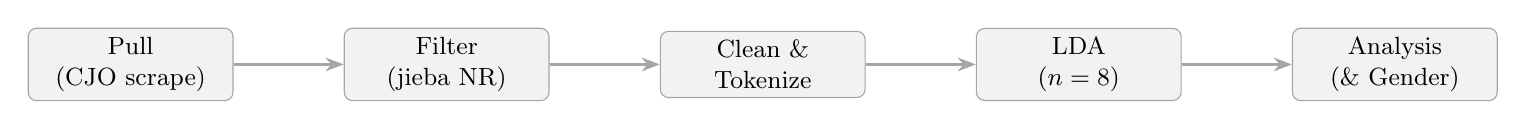
\begin{tikzpicture}[
  node distance=0.8cm and 1.4cm,
  box/.style={rectangle, rounded corners=3pt, draw=gray!70, fill=gray!10,
              minimum width=2.6cm, minimum height=0.7cm, font=\small, align=center},
  arrow/.style={-Stealth, thick, gray!70}
]
  \node[box] (pull)    {Pull\\(CJO scrape)};
  \node[box, right=of pull] (filter)  {Filter\\(jieba NR)};
  \node[box, right=of filter] (clean)   {Clean \&\\Tokenize};
  \node[box, right=of clean] (lda)     {LDA\\($n=8$)};
  \node[box, right=of lda] (results) {Analysis\\(\& Gender)};

  \draw[arrow] (pull)   -- (filter);
  \draw[arrow] (filter) -- (clean);
  \draw[arrow] (clean)  -- (lda);
  \draw[arrow] (lda)    -- (results);
\end{tikzpicture}
\caption{Analysis pipeline. Each stage corresponds to a numbered notebook in the repository.}
\label{fig:pipeline}
\end{figure}

\subsection{Text Cleaning and Tokenization}

Because court cases are retrieved as raw Chinese text, preprocessing focused on removing legal boilerplate that would dominate topic distributions without conveying substantive complaint content. A custom stopword list of 152 terms was developed iteratively: an initial set covered standard legal procedural phrases (\begin{CJK}{UTF8}{gbsn}一审、被告、诉讼费\end{CJK}, etc.), then extended after inspecting top keywords from the initial LDA visualization. The list includes terms like \begin{CJK}{UTF8}{gbsn}送达\end{CJK} (service of process), \begin{CJK}{UTF8}{gbsn}出生\end{CJK} (birth, appearing in case headers), and \begin{CJK}{UTF8}{gbsn}申请\end{CJK} (application)---all high-frequency but semantically uninformative.

After stopword removal, each document was tokenized using jieba's \texttt{extract\_tags} function (TF-IDF keyword extraction), retaining the top 50 keywords per case with allowed parts of speech: nouns (n, nt, nz), verbs (v, vn), and adjectives (a). Tokens shorter than two characters were discarded to reduce single-character noise.

\subsection{Selecting the Number of Topics}

To choose the optimal number of topics $k$, I evaluated models for $k = 2$ to $15$ along two metrics: (1) mean pairwise Jaccard overlap between topic keyword lists (lower is better, indicating distinct topics) and (2) semantic coherence using the Gensim $C_v$ coherence model (higher is better). The optimal $k$ was selected as the value maximizing the difference $C_v(k) - \overline{J}(k)$.

As shown in Figure~\ref{fig:ntopics}, $k = 8$ yields the best balance, with coherence exceeding topic overlap by the widest margin. This configuration was used for all subsequent analysis.

\begin{figure}[H]
  \centering
  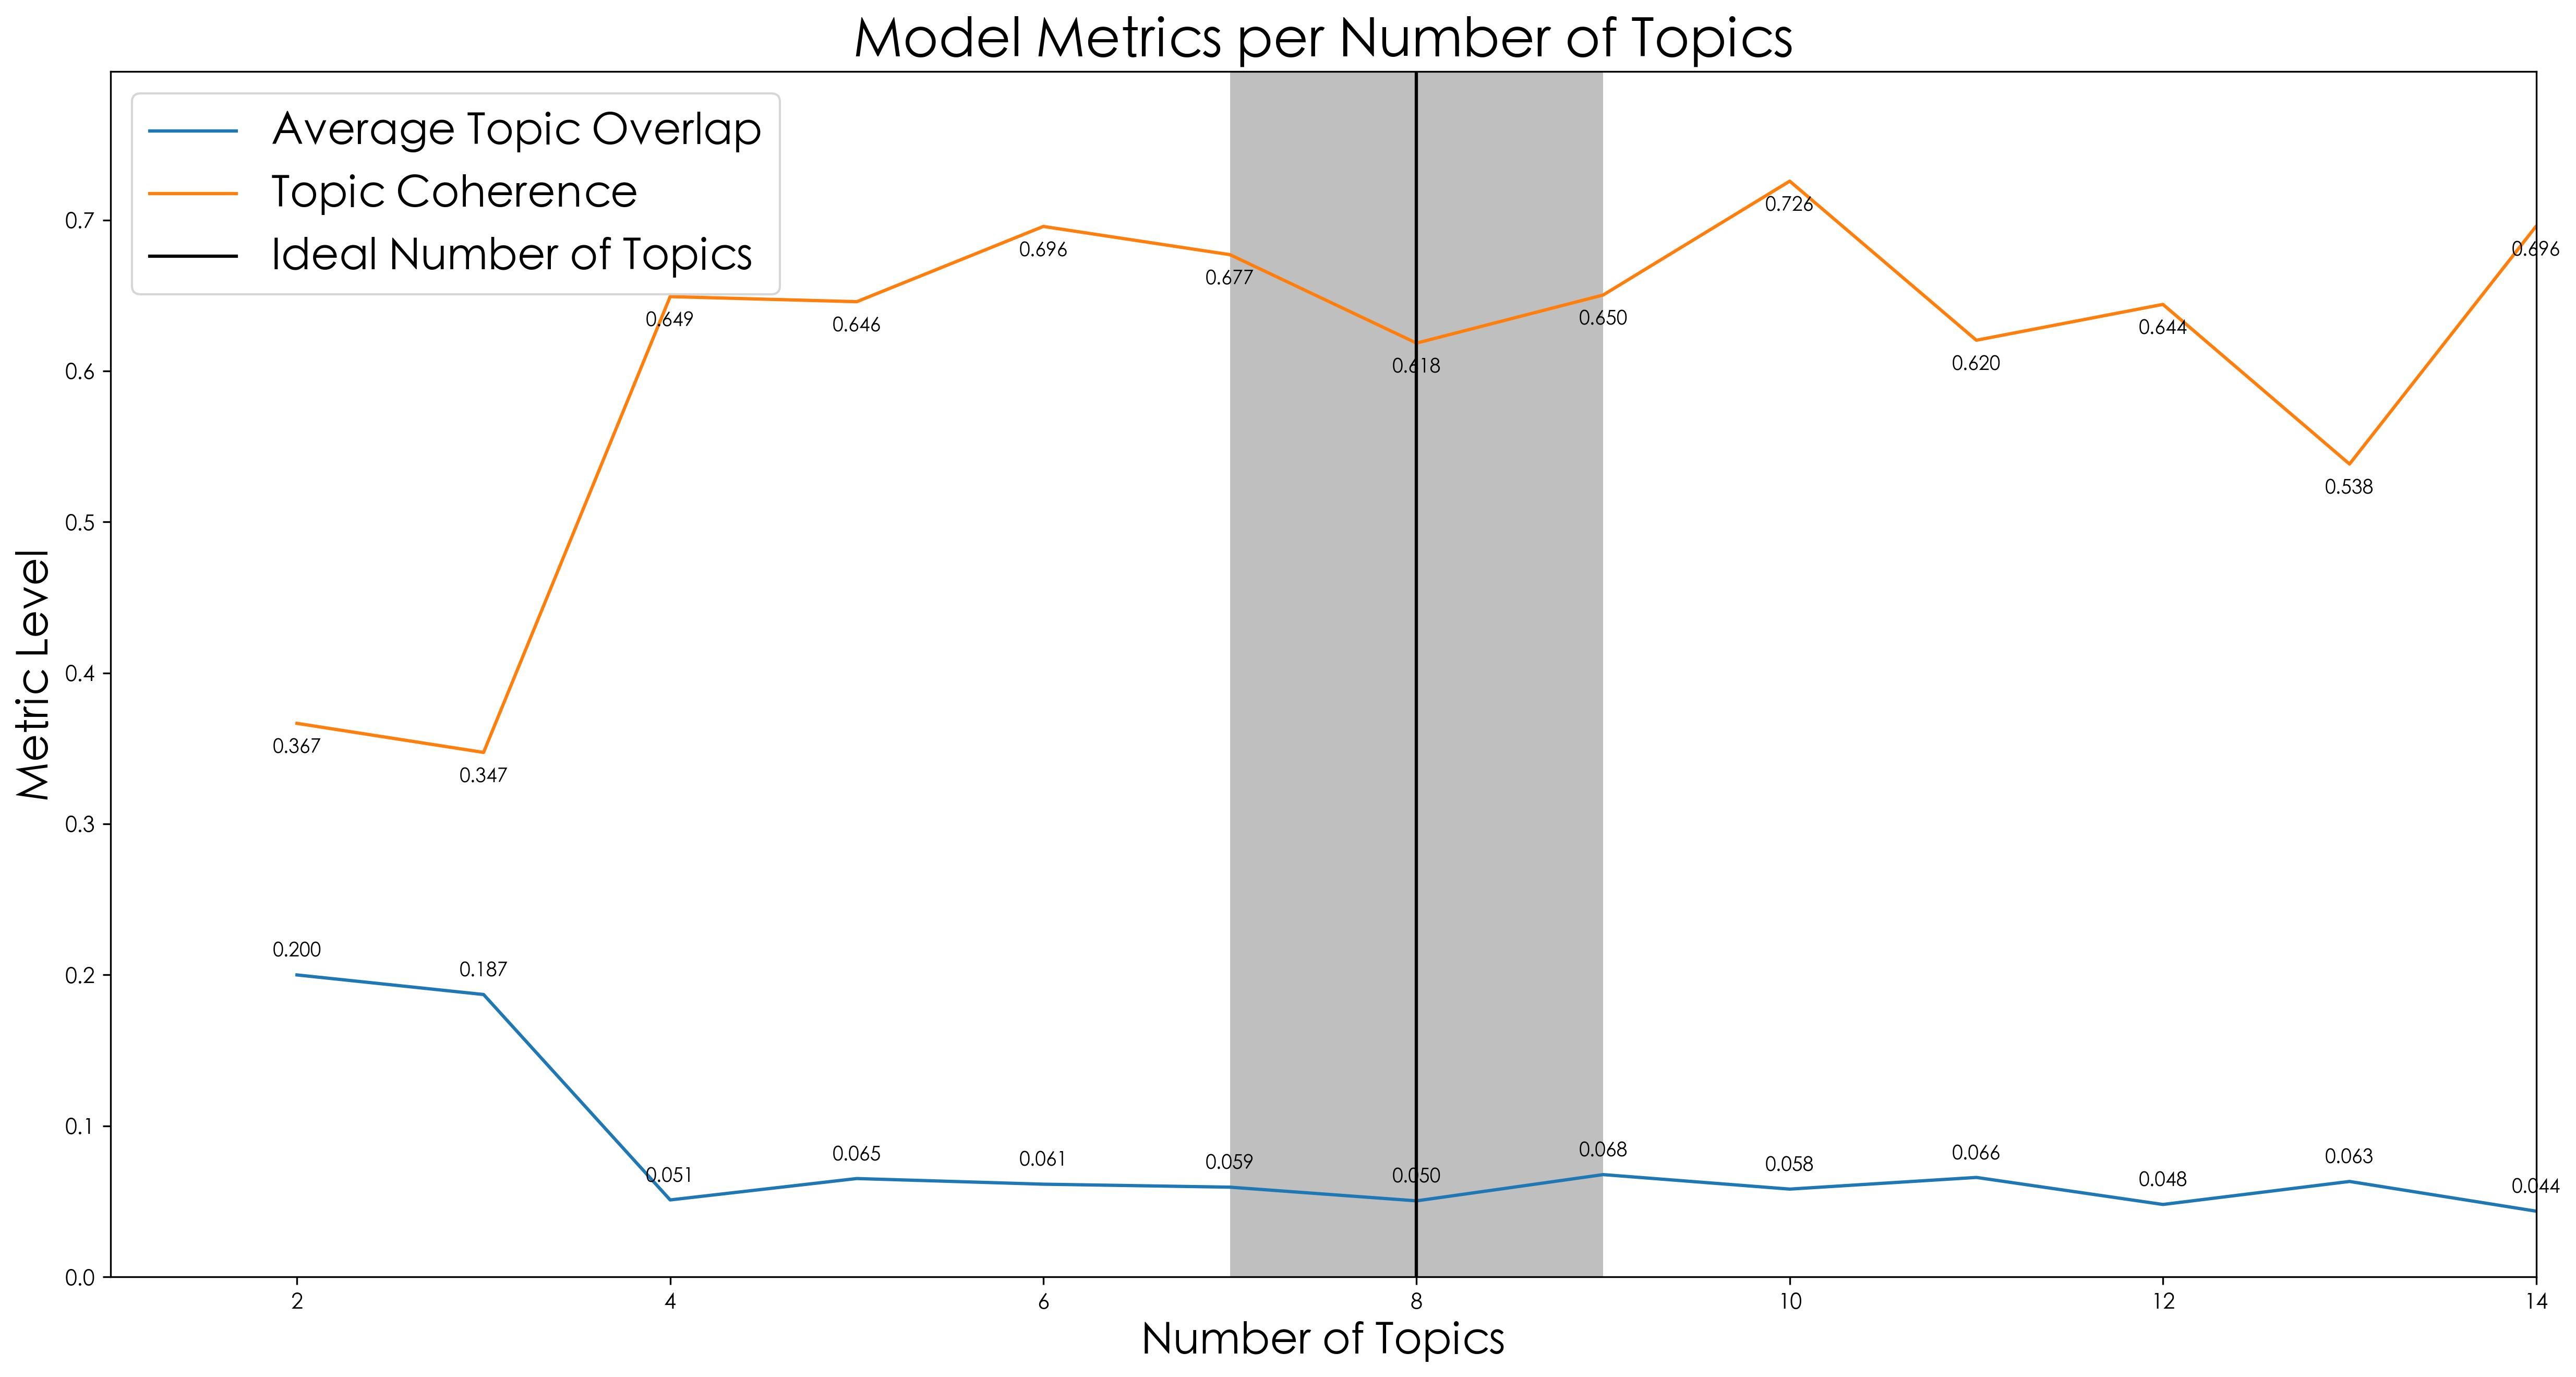
\includegraphics[width=0.85\linewidth]{output/n_topic_comparison.jpeg}
  \caption{Topic coherence ($C_v$) and mean pairwise Jaccard overlap as a function of the number of topics $k$. The vertical line marks $k = 8$, which maximizes the coherence-overlap gap.}
  \label{fig:ntopics}
\end{figure}

\subsection{LDA Topic Modeling and Identification}

Latent Dirichlet Allocation was estimated using the Gensim LDA implementation \citep{gensim} with $k = 8$, 15 passes, symmetric Dirichlet $\alpha$, and a fixed random seed for reproducibility. The vocabulary was filtered to terms appearing in at least 5\% and at most 95\% of documents, reducing the dictionary from 2,009 to 216 unique terms.

Topic identification followed a two-step procedure. First, topics were ranked by corpus share using pyLDAvis \citep{sievert2014}. Second, substantive theme labels were assigned using \textit{loglift}-ranked terms (which surface terms exclusive to a topic rather than terms that are merely frequent), cross-checked against frequency-ranked terms to confirm the interpretation. Claude Code was used to assist in reading the raw LDA visualization HTML and proposing initial theme labels; all labels and stopword decisions were reviewed and finalized manually (see Appendix).

%% ─────────────────────────────────────────────────────
\section{Results}

\subsection{Eight Principal Topics}

Table~\ref{tab:topics} presents the eight topics identified by the model, ordered by corpus share. Each entry includes the Chinese and English topic label, the corpus percentage, and the top five loglift-ranked terms.

\begin{table}[H]
\centering
\caption{LDA topic summary for the 8-topic model ($n = 79$ cases). Corpus \% = share of the total corpus attributed to each topic by the model. Top terms are ranked by loglift (exclusivity over frequency).}
\label{tab:topics}
\renewcommand{\arraystretch}{1.25}
\resizebox{\linewidth}{!}{%
\begin{tabular}{@{}clclp{5.2cm}@{}}
\toprule
\textbf{Topic} & \textbf{Corpus \%} & \textbf{Cluster} & \textbf{English Label} & \textbf{Top Terms (loglift)} \\
\midrule
T1 & 21.9\% & Sports — Personnel & Sports-Team Roster Mgmt.\ \& Wage Disputes &
  \begin{CJK}{UTF8}{gbsn}在编, 欠款, 违纪, 体委, 离队\end{CJK} \\
T2 & 21.7\% & Commercial & Commercial Contract Breach \& Debt Recovery &
  \begin{CJK}{UTF8}{gbsn}公司财务, 补救措施, 经手人, 补充协议, 兽药\end{CJK} \\
T3 & 16.3\% & Sports — Medical & General Athlete Compensation \& Medical Costs &
  \begin{CJK}{UTF8}{gbsn}住宿费, 椎间盘, 工作队, 食宿费, 法律效力\end{CJK} \\
T4 & 13.6\% & Sports — Medical & Work Injury Insurance \& Employment Termination &
  \begin{CJK}{UTF8}{gbsn}工伤保险, 书面通知, 赔偿金, 伤病, 辞退\end{CJK} \\
T5 &  9.5\% & Commercial — Rights & Online Infringement \& Athlete Image-Rights &
  \begin{CJK}{UTF8}{gbsn}财产损失, 肖像权, 百科, 致歉, 二维码\end{CJK} \\
T6 &  9.3\% & Sports — Personnel & Administrative Litigation Procedure &
  \begin{CJK}{UTF8}{gbsn}行政诉讼法, 体工, 起诉状, 签收, 三性\end{CJK} \\
T7 &  4.3\% & Sports — Medical & Sports Training Injuries \& Social Insurance &
  \begin{CJK}{UTF8}{gbsn}体育运动, 木樨园, 工龄, 半月板, 社会保险\end{CJK} \\
T8 &  3.4\% & Sports — Personnel & Statute of Limitations \& Retirement Placement &
  \begin{CJK}{UTF8}{gbsn}时效, 垒球, 全运会, 扣发, 主体资格\end{CJK} \\
\bottomrule
\end{tabular}}
\end{table}

\subsection{Sports-Specific Disputes Dominate}

Aggregating by cluster (Figure~\ref{fig:pie}), \textbf{68.8\%} of the corpus concerns sports-career disputes: personnel and administrative issues account for 34.6\% (T1, T6, T8), while medical and injury claims account for 34.2\% (T3, T4, T7). The remaining \textbf{31.2\%} is commercial or financial in nature (T2, T5).

The dominance of sports-specific disputes is notable given that all athletes in this corpus are technically \textit{retired}. The persistence of employment, wage, and injury grievances after career end reflects structural features of the jǔguó tǐzhì: athletes employed as state workers (编制) retain legal entitlements---and disputes---tied to their in-service status long after they leave active competition. T1's high-loglift debt terms (\begin{CJK}{UTF8}{gbsn}欠款, 清偿, 年利率\end{CJK}) alongside sports-HR vocabulary (\begin{CJK}{UTF8}{gbsn}在编, 体委, 人事处\end{CJK}) suggest that many cases involve unpaid wages or back-pay settlements framed within formal HR adjudication proceedings.

T4 (Work Injury Insurance \& Employment Termination, 13.6\%) is distinct from the broader medical cluster (T3) in its emphasis on \textit{formal dismissal procedures}: \begin{CJK}{UTF8}{gbsn}辞退\end{CJK} (termination), \begin{CJK}{UTF8}{gbsn}书面通知\end{CJK} (written notice), and \begin{CJK}{UTF8}{gbsn}停发\end{CJK} (suspension of payment) all rank highly. Athletes in this cluster appear to be disputing both the sports-injury origin of their disability and the lawfulness of the processes by which they were removed from employment.

\begin{figure}[H]
  \centering
  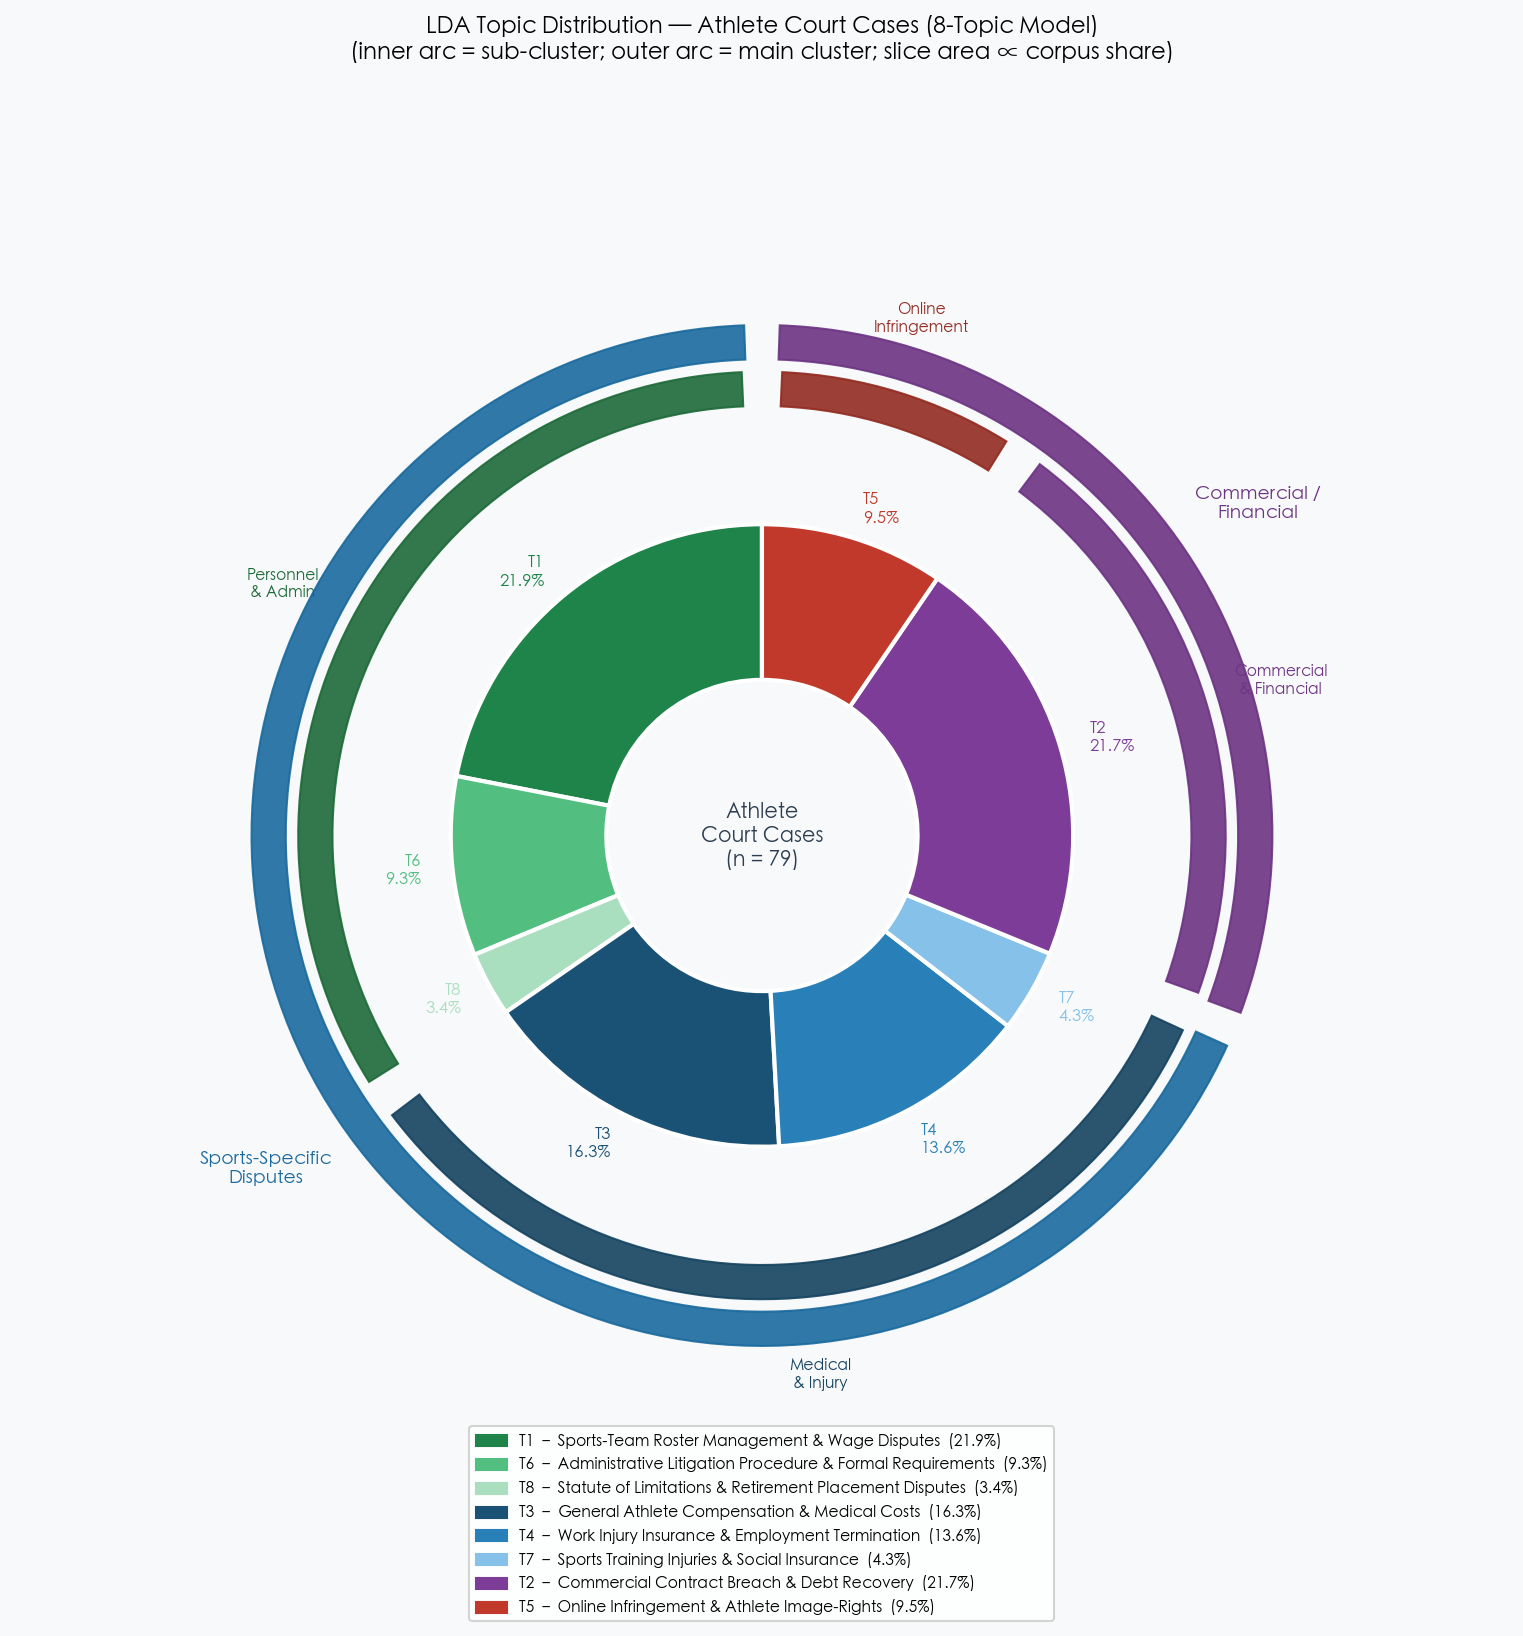
\includegraphics[width=0.82\linewidth]{output/topic_pie_n8.png}
  \caption{LDA topic distribution for the 8-topic model ($n = 79$ cases). Inner arc = sub-cluster; outer arc = main cluster. Slice area is proportional to corpus share.}
  \label{fig:pie}
\end{figure}

\subsection{Online Rights Infringement: An Understudied Category}

Topic T5 (Online Infringement \& Athlete Image-Rights, 9.5\%) warrants separate attention because it is topically unlike the other seven topics. The defining loglift terms---\begin{CJK}{UTF8}{gbsn}肖像权\end{CJK} (portrait rights), \begin{CJK}{UTF8}{gbsn}百科\end{CJK} (online encyclopedia), \begin{CJK}{UTF8}{gbsn}二维码\end{CJK} (QR code), \begin{CJK}{UTF8}{gbsn}截图\end{CJK} (screenshot), \begin{CJK}{UTF8}{gbsn}微信\end{CJK} (WeChat)---describe the unauthorized commercial use of athlete likeness through digital channels. Plaintiffs in these cases seek formal apologies (\begin{CJK}{UTF8}{gbsn}致歉\end{CJK}) and compensation for both material and dignitary losses (\begin{CJK}{UTF8}{gbsn}财产损失, 抚慰金\end{CJK}), with claims grounded in China's Tort Liability Law (\begin{CJK}{UTF8}{gbsn}责任法\end{CJK}).

Image-rights disputes are commonly associated with celebrities; the finding that nearly one in ten athlete cases falls into this category suggests that retired athletes face a form of commercial exploitation of their public identity that the existing welfare literature has largely overlooked.

\subsection{Keyword Distribution Across Topics}

Figure~\ref{fig:keywords} shows the top 15 corpus-wide keywords by document frequency, with each bar segmented by topic attribution via $p(\text{topic} | \text{term})$ from the LDA model. Several patterns are notable.

\begin{CJK}{UTF8}{gbsn}体育局\end{CJK} (Sports Bureau) is the single most frequent term, appearing in 33 of 79 cases, and distributes across all personnel and medical topics---confirming the Sports Bureau as the primary institutional defendant across dispute types. \begin{CJK}{UTF8}{gbsn}国家体育总局\end{CJK} (General Administration of Sport, China's apex sports authority) appears almost exclusively in T4, suggesting that work-injury insurance claims more often reach the national level. The term \begin{CJK}{UTF8}{gbsn}微信\end{CJK} (WeChat, rank 14) is an anomaly in the keyword list: it is almost entirely attributed to T5, confirming that its high document frequency reflects a concentrated cluster of image-rights cases rather than ubiquitous usage across the corpus.

\begin{figure}[H]
  \centering
  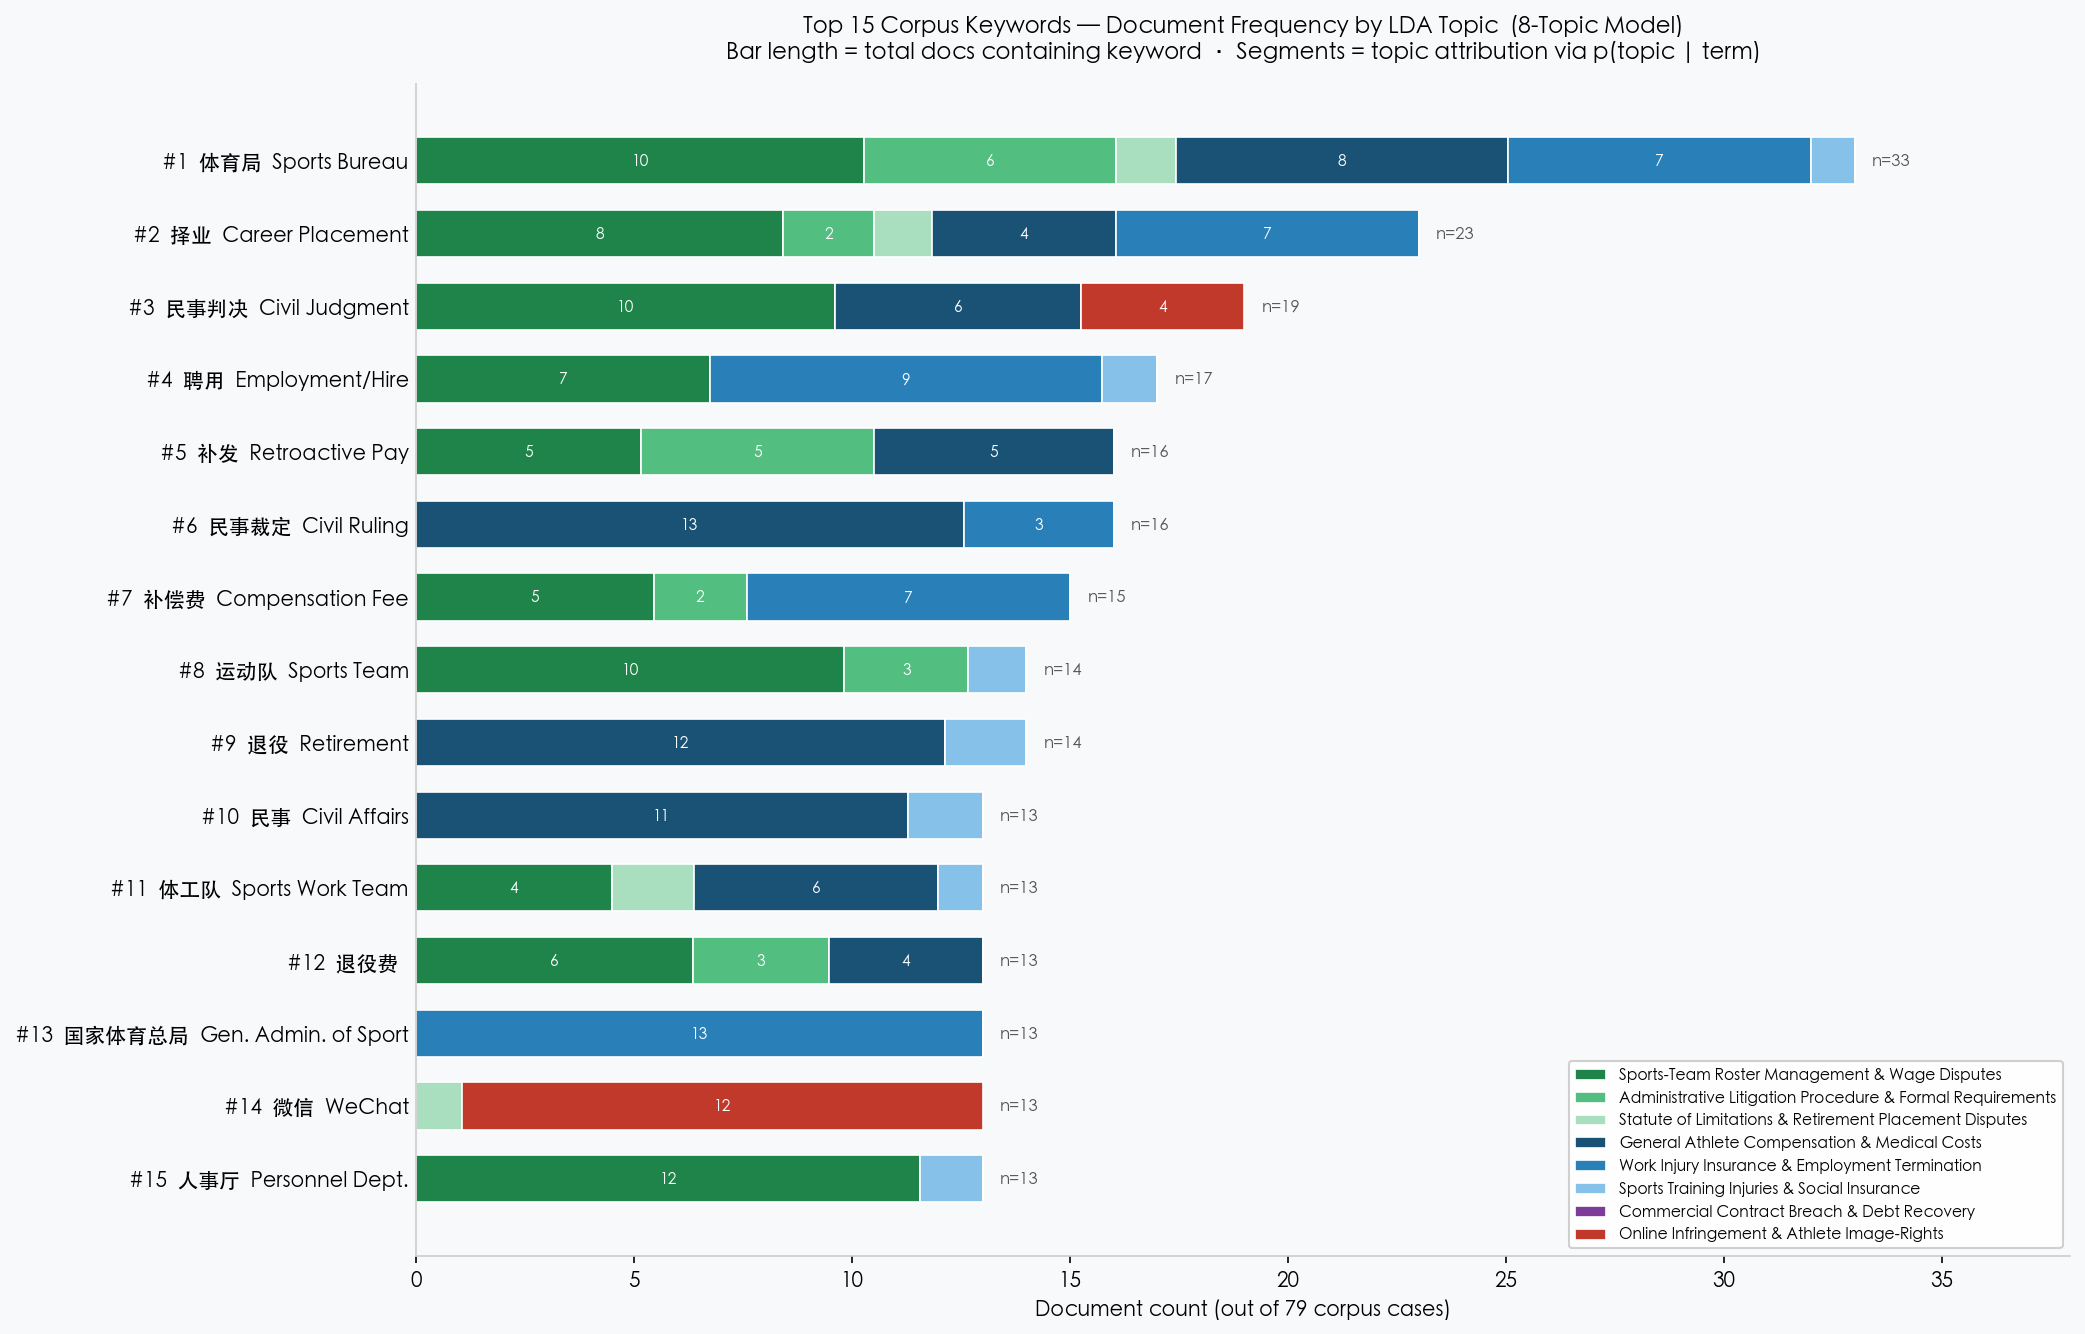
\includegraphics[width=\linewidth]{output/keyword_distrib.png}
  \caption{Top 15 corpus keywords by document frequency ($n = 79$). Bar length = total documents containing the keyword. Segments show topic attribution via $p(\text{topic} | \text{term})$. Inline numbers indicate absolute document count per segment where $\geq 2$.}
  \label{fig:keywords}
\end{figure}

%% ─────────────────────────────────────────────────────
\section{Supplementary Findings: Gender and Judicial Visibility}

Male judicial visibility is consistently higher than female in general-population studies of court behavior---a pattern attributed to differences in legal awareness, income, and social support \citep{gallagher2006}. I was curious whether this pattern holds within the retired-athlete context, where female athletes represent a sizeable share of elite participants.

Gender was identified from the litigant line of each case header. Chinese court documents routinely disclose the party's name, gender, date of birth, and ethnicity in the opening paragraph. Of the 79 total cases, \textbf{21} had no identifiable gender marker---primarily cases involving institutional plaintiffs or pseudonymized individuals---leaving 58 cases for gender analysis. Of these, \textbf{42 (72.4\%) named male litigants} and \textbf{19 (27.6\%) named female litigants}, representing a 38\% gap in female judicial visibility relative to male (Figure~\ref{fig:gender}).

\begin{figure}[H]
  \centering
  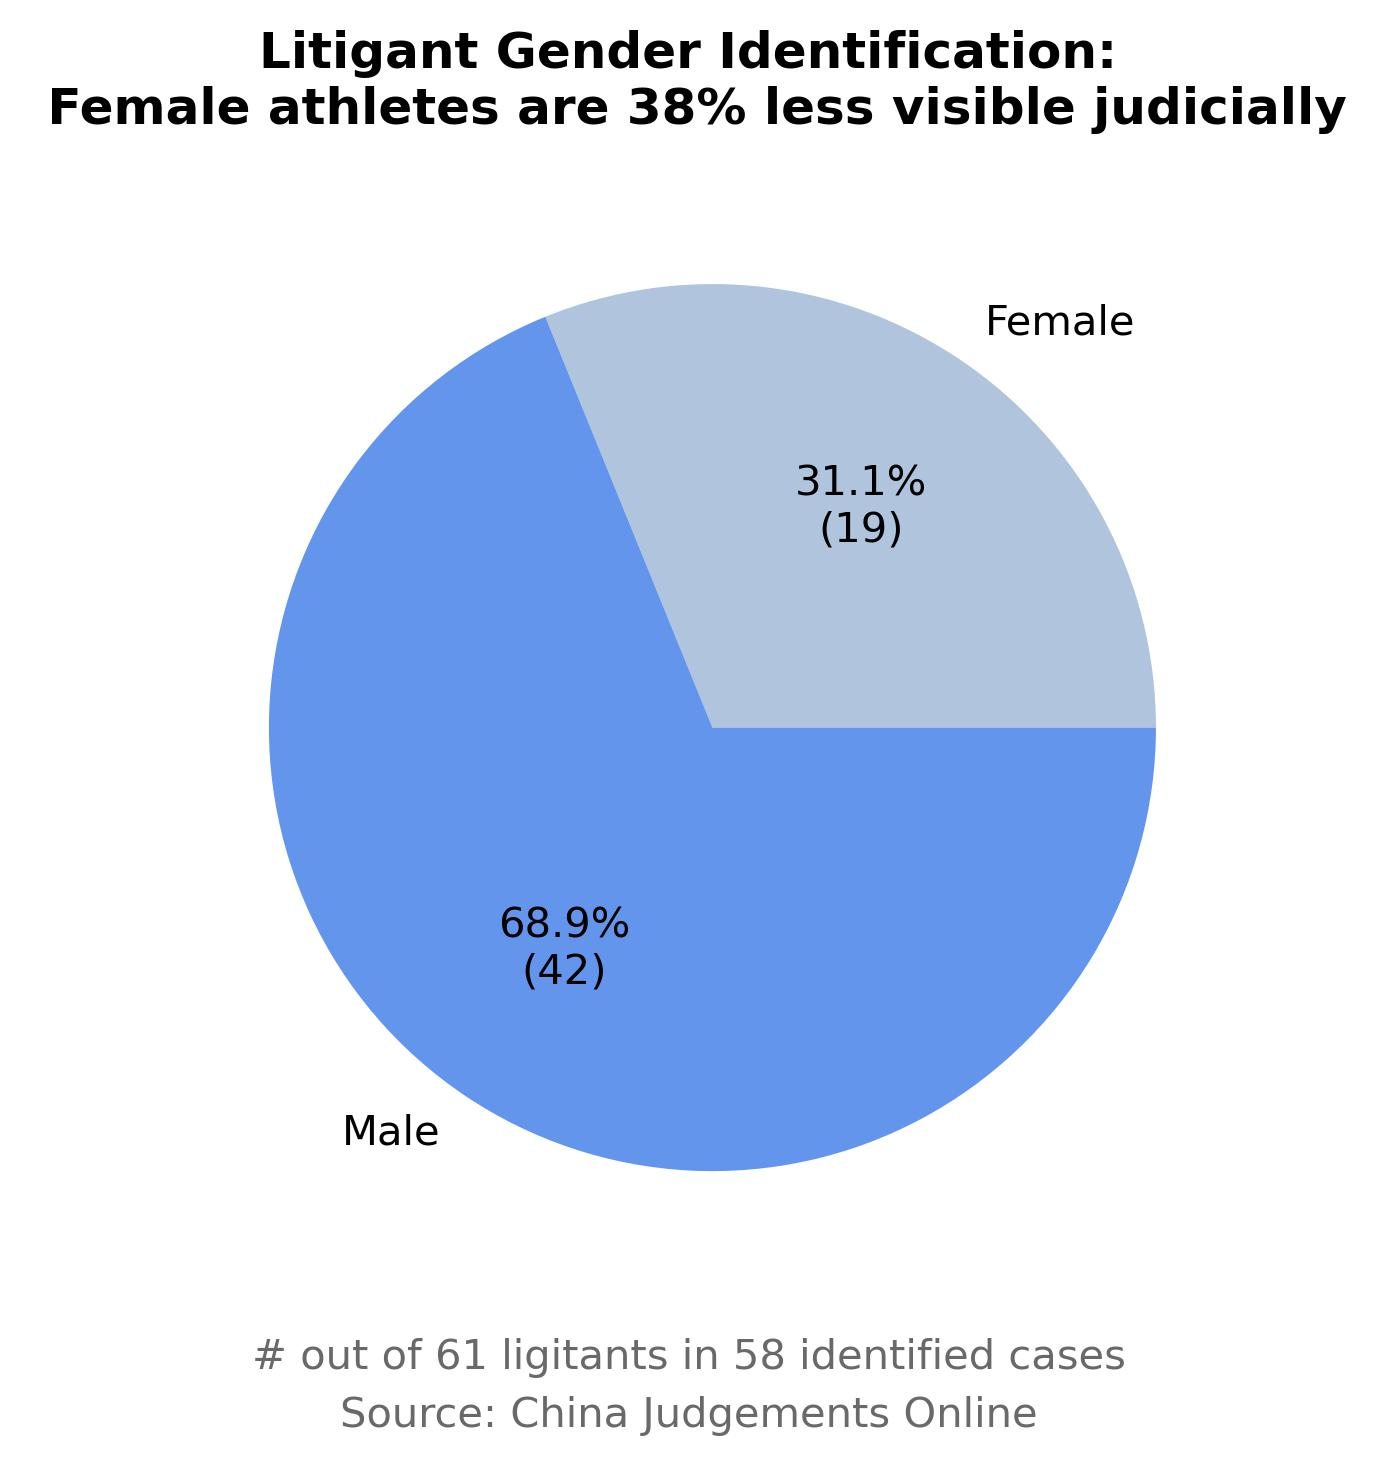
\includegraphics[width=0.55\linewidth]{output/gender_dif.jpeg}
  \caption{Litigant gender distribution among the 58 cases with identifiable gender ($n_\text{male}=42$, $n_\text{female}=19$). Female athletes are 38\% less judicially visible than male.}
  \label{fig:gender}
\end{figure}

Because male athletes outnumber female athletes in China's sports system overall \citep{csb2022}, the observed gap may partly reflect demographic composition rather than differential propensity to litigate. Nevertheless, the disparity is consistent with cross-national findings on gender and court access, and the legal challenges faced by female retired athletes are by no means absent from the data.

%% ─────────────────────────────────────────────────────
\section{Discussion}

\paragraph{Main findings.}
LDA topic modeling on 79 court cases from CJO reveals a coherent picture of what retired Chinese athletes fight for: the majority of grievances are rooted in the career structure they inhabited as active athletes. Personnel disputes---unpaid wages, improper dismissal, failure to honor retirement placement---account for over a third of cases, as do medical and injury claims. This is not surprising given the physical demands of elite Chinese sport and the blurry boundary between the athlete's person and the state employer. What is more surprising is the commercial cluster: a 21.7\% share of commercial contract disputes positions sports-affiliated entities as active participants in commercial life, not merely welfare recipients, while the 9.5\% image-rights cluster signals a genuinely under-researched avenue of athlete exploitation.

\paragraph{Limitations.}
The corpus is small (79 cases) and limited to cases that made it to formal adjudication and into the public database. CJO has faced documented take-downs and selective publication \citep{clarke2023}, and many grievances likely never reach litigation. The topical composition observed here reflects the intersection of actual complaint patterns and willingness to litigate, compounded by what CJO chooses to publish. Generalizability to the full population of retired athlete grievances is therefore limited.

\paragraph{Keyword reliability.}
As noted in the discussion of Figure~\ref{fig:keywords}, certain terms---most prominently \begin{CJK}{UTF8}{gbsn}微信\end{CJK} (WeChat)---are interpretable as topic markers only in context; isolated from their case narrative, they would appear semantically promiscuous. The LDA model handles this correctly at the corpus level (WeChat concentrates in T5), but individual keyword attribution via $p(\text{topic} | \text{term})$ should be treated with caution for terms that plausibly appear across contexts.

\paragraph{Future directions.}
The agentic AI analysis conducted during this project (see Appendix) identified topics that merit deeper investigation: the administrative procedure topic (T6) in particular---centered on formal litigation requirements (\begin{CJK}{UTF8}{gbsn}起诉状\end{CJK}, \begin{CJK}{UTF8}{gbsn}三性\end{CJK} admissibility, standing challenges)---suggests that athletes may face systematic procedural barriers to accessing judicial redress, a question amenable to further qualitative coding. Linking court outcomes (case won/lost) to topic clusters would test whether certain complaint types are systematically dismissed, providing a more direct measure of welfare system failure.

%% ─────────────────────────────────────────────────────
\bibliographystyle{plainnat}
\begin{thebibliography}{99}

\bibitem[Clarke(2023)]{clarke2023}
Donald Clarke.
\newblock Follow-up on the fate of China Judgments Online.
\newblock \textit{The China Collection}, 2023.
\newblock URL: \url{https://thechinacollection.org/follow-fate-china-judgments-online/}.

\bibitem[CSB(2022)]{csb2022}
China Sports Bureau.
\newblock \textit{National Sports Industry Development Statistics}, 2022.
\newblock Beijing: General Administration of Sport of China.

\bibitem[Gallagher(2006)]{gallagher2006}
Mary E.~Gallagher.
\newblock Mobilizing the law in China: ``informed disenchantment'' and the development of legal consciousness.
\newblock \textit{Law \& Society Review}, 40(4):783--816, 2006.

\bibitem[{Jieba Contributors}(2023)]{jieba}
{Jieba Contributors}.
\newblock \textit{Jieba: Chinese Text Segmentation}.
\newblock Version 0.42.1, 2023.
\newblock URL: \url{https://github.com/fxsjy/jieba}.

\bibitem[Liu(2014)]{liu2014}
Jian Liu.
\newblock Retirement welfare for elite athletes in China: Policy framework and implementation gaps.
\newblock \textit{International Journal of Sport Policy and Politics}, 6(3):367--384, 2014.

\bibitem[{\v{R}}eh{\r{u}}{\v{r}}ek and Sojka(2010)]{gensim}
Radim {\v{R}}eh{\r{u}}{\v{r}}ek and Petr Sojka.
\newblock Software framework for topic modelling with large corpora.
\newblock In \textit{Proceedings of the LREC 2010 Workshop on New Challenges for NLP Frameworks}, pages 45--50, 2010.

\bibitem[Sievert and Shirley(2014)]{sievert2014}
Carson Sievert and Kenneth Shirley.
\newblock LDAvis: A method for visualizing and interpreting topics.
\newblock In \textit{Proceedings of the Workshop on Interactive Language Learning, Visualization, and Interfaces}, pages 63--70, 2014.

\bibitem[Xinhua(2016)]{xinhua2016}
Xinhua News Agency.
\newblock Retired athletes face difficult transitions as welfare gaps persist.
\newblock \textit{Xinhua}, September 2016.

\bibitem[Xu(2008)]{xu2008}
Guoqi Xu.
\newblock \textit{Olympic Dreams: China and Sports, 1895--2008}.
\newblock Harvard University Press, 2008.

\end{thebibliography}

%% ─────────────────────────────────────────────────────
\newpage
\appendix
\section*{Appendix: Agentic Analysis --- AI Transcript and Critical Reflection}

\subsection*{What I Used AI For}

AI assistance (Claude Code via the Claude Code CLI) was used at two stages of this project: (1) stopword refinement after an initial LDA run, and (2) topic identification from the LDA visualization.

\paragraph{Stage 1: Stopword Refinement.}
After running an initial LDA model, I shared the raw CSV of filtered cases and the HTML LDA visualization with Claude Code and asked it to propose boilerplate terms for the stopword list. The model proposed 11 terms:

\begin{center}
\begin{CJK}{UTF8}{gbsn}民事判决, 民事裁定, 民事, 出生, 汉族, 送达, 公告送达, 案件, 申请, 规定, 京民\end{CJK}
\end{center}

I accepted seven of these additions: \begin{CJK}{UTF8}{gbsn}出生, 送达, 公告送达, 案件, 申请, 规定, 京民\end{CJK}. These are indeed procedural boilerplate with no substantive content.

I rejected four: \begin{CJK}{UTF8}{gbsn}民事判决\end{CJK} (civil judgment), \begin{CJK}{UTF8}{gbsn}民事裁定\end{CJK} (civil ruling), \begin{CJK}{UTF8}{gbsn}民事\end{CJK} (civil), and \begin{CJK}{UTF8}{gbsn}汉族\end{CJK} (Han ethnicity). The civil-procedure terms are important \textit{case-type} signals---they distinguish between substantive judgments and procedural rulings, which is legally meaningful. \begin{CJK}{UTF8}{gbsn}汉族\end{CJK} provides demographic information about the litigant pool that may be analytically relevant in future work.

\paragraph{Stage 2: Topic Identification.}
I fed Claude Code the rendered HTML LDA visualization (\texttt{lda\_vis\_chn\_8.html}) and asked it to identify substantive themes for each display topic using loglift-ranked terms. The model produced initial topic labels that I cross-checked against the frequency-ranked terms and sample case text.

\subsection*{What I Accepted and Why}

The topic label framework the model proposed---distinguishing personnel/admin, medical/injury, commercial, and rights sub-clusters---was well-aligned with my own reading of the keywords and was accepted with minor wording edits. The AI's identification of Topic T5 as an image-rights cluster was particularly useful: I initially read the \begin{CJK}{UTF8}{gbsn}微信\end{CJK}/\begin{CJK}{UTF8}{gbsn}截图\end{CJK}/\begin{CJK}{UTF8}{gbsn}百科\end{CJK} keyword cluster as a general digital-evidence topic, and the model's framing around \begin{CJK}{UTF8}{gbsn}肖像权\end{CJK} (portrait rights) and the commercial exploitation of athlete likeness was more precise.

\subsection*{What I Rejected and Where the Assistant Went Wrong}

The AI's proposed grouping of Topic T2 (Commercial Contract \& Debt Recovery) under ``sports-specific disputes'' was incorrect. The defining vocabulary of T2---\begin{CJK}{UTF8}{gbsn}公司财务, 经手人, 兽药, 蔬菜水果\end{CJK}---reflects generic commercial operations (veterinary drugs, produce, company finance) with no sports-specific content. I reclassified T2 under the ``Commercial/Financial'' cluster.

More broadly, as noted in the Discussion section, the AI identified \begin{CJK}{UTF8}{gbsn}微信\end{CJK} (WeChat) as a primary driver of the image-rights topic. While correct at the topic level, WeChat is in fact a general-purpose communication application. The keyword distribution analysis (Figure~\ref{fig:keywords}) shows that WeChat's concentration in T5 is a corpus-level pattern, but at the individual-case level it could appear in any context. This is a known limitation of bag-of-words approaches: single-term attribution does not account for the semantic role of a word within its context.

\subsection*{Reflection}

The AI was most useful as a first-pass analyst for structured text---it reliably extracted and organized keyword information from the LDA HTML that would have taken me considerably longer to parse manually. Where it struggled was in interpretive tasks requiring domain knowledge (Chinese sports law, the jǔguó tǐzhì institutional structure) and in distinguishing between a term's statistical association with a topic versus its substantive relevance to the underlying dispute. Human review remained essential for every classification decision.

\end{document}
